\section{Optimal Travel via Macro-Edges}
After interior nodes are eliminated, macro-edges have to be added between perimeter
nodes to ensure rectangles are traversed optimally.
We will describe a strategy that adds only \emph{non-dominated} macro edges; i.e. edges whose 
lengths are strictly less than the length of any alternative path between the same pair of nodes.
There are three cases to discuss. In each case the length of each added macro-edge 
is equal to the heuristic (or Octile) distance between its two endpoints.
\par 
\textbf{Case 1:} nodes on the same side of the perimeter are connected
just as in the original grid.
\textbf{Case 2:} nodes on orthogonal sides of the perimeter are connected \emph{iff} the shortest path between them is a diagonal
(45-degree) line; this is illustrated in Figure \ref{fig-macroedges} (a).
\textbf{Case 3:} nodes on opposite sides of the perimeter. 
For each such node we generate a ``fan'' of neighbours from the opposite side; this is shown in Figure
\ref{fig-macroedges} (b).
Starting from a node such as $t_{1}$ we step to the closest
neighbour from the opposite side and extend the fan away
from the middle, adding each node we encounter.  The last node
on either side of the fan is placed diagonally, at 45 degrees, from $t_{1}$
(such as $t_{2}$) or located in the corner of the perimeter (whichever is encountered first).  
Other nodes, such as $t_{3}$, can be reached optimally via the path $\langle t_1, t_2, \dots,
t_3 \rangle $.

\begin{lemma} \label{lemma-rooms} Let $R$ be an empty rectangle in
an 8-connected grid map. Let $m$ and $n$ be two perimeter locations.
Then, $m$ and $n$ can be connected optimally through a path that
contains only non-dominated macro-edges.
\end{lemma}

\begin{proof}:
We split the proof over the 3 cases discussed earlier.
In the first case we walk along the perimeter from $m$ to $n$; the
optimality of this path is immediate. In the second and third case 
the two nodes can be connected through an optimal path that has one diagonal macro-edge
(at one end of the path) and zero or more straight macro-edges.
See again the example of travelling from $t_1$ to $t_3$ in Figure
\ref{fig-macroedges} (b).
\end{proof}

\begin{figure}[tb]
       \begin{center}
		   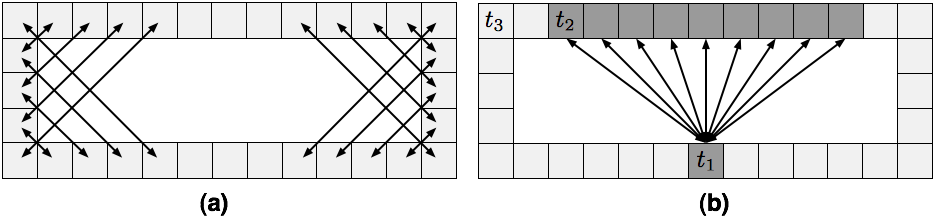
\includegraphics[width=0.97\columnwidth, trim = 10mm 10mm 10mm 0mm]
			{diagrams/macroedges_wide.png}
       \end{center}
	\vspace{-3pt}
       \caption{(a) Macro edges between nodes on orthogonal sides of an empty
       rectangle. (b) Each node on the perimeter is connected to a set of 
		nodes on the opposite side.}
       \label{fig-macroedges}
\end{figure}

\noindent
\textbf{Node Insertion:}
When the start or goal is located in the interior of an empty rectangle
we will temporarily re-insert them into the graph for the duration of a search.
{If the start and goal are from the same room no insertion is necessary; an optimal path is trivially
available. } {Otherwise, we add four ``fans'' (collections) of macro edges.  Each fan connects
the start (goal) node to a set of nodes on one side of the rectangle's
perimeter.  Fans are built as shown earlier.}
To prove optimality we run the argument given
for Case 3 of Lemma \ref{lemma-rooms}, substituting $m$ for the newly inserted node.
%\par
%Given the simple geometry of rectangles, it is possible to identify in constant
%time the set of nodes which the start or goal must be connected to.  Further,
%these successors could be generated on-the-fly.

%We claim that using the temporary macro edges added by this algorithm it is possible to travel optimally from the start or goal 
%location to any node on the perimeter of the start or goal rectangle. 
%\par \noindent
%\newline
\begin{theorem}
For every optimal path $\pi$ on an original grid, there exists an optimal path
$\pi'$ on the reformulated grid such that $\pi$ and $\pi'$ have the
same cost.
\end{theorem}
\begin{proof}
Consider a rectangle R that is crossed by an optimal path $\pi$ in the original grid.
Let $m$ and $n$ be the two perimeter points along $\pi$.
According to Lemma~\ref{lemma-rooms}, there is a way to connect $m$ and $n$
optimally in the modified graph. Thus, we replace the original path segment $\langle m,
\dots, n\rangle$ in $\pi$ with a cost-wise equivalent from the
modified grid.  The case when $m$ (or $n$) is the start or goal node is
addressed similarly.  By performing such a
replacement for all rectangles intersected by $\pi$, we obtain a
path $\pi'$ that satisfies the desired properties.
\end{proof}

%\textbf{Optimality:} We claim the symmetry elimination procedure outlined in this section is sufficient to guarantee
%that A*, running on a modified 8-connected grid map, will always find an optimal length solution if one exists.
%Our argument follows from Lemma \ref{lemma-rooms} and Lemma \ref{lemma-insertion}.
%It is based on the observation that for every segment of an optimal length path, which enters a rectangle at some node $m$,
%traverses through the interior of the rectangle and exits at some node $n$, there is an equivalent length path that mentions only 
%nodes from the perimeter of that rectangle and possibly one macro edge.

